\documentclass{beamer}
\usetheme{boadilla}
%\usepackage[scale]{helvet}
\usepackage{etex}
\usepackage{helvet}
\usepackage{translator}

\usepackage[all]{xy}
\usepackage{color}
\usepackage{booktabs}
\usepackage{amsmath,amsthm,amssymb}

\usepackage{fancybox}
\usepackage{comment}
\usepackage{array}
\usepackage{multicol}
\usepackage{multirow}
\usepackage[export]{adjustbox} %for alignment

%% I like helvetica, but here are some other font options
% \usepackage{libertine}
%\usepackage{xunicode}
%\usepackage{xltxtra}
%\usepackage{fontspec}
%\setmainfont{Minion Pro}
%\xyoption{color}
%\xyoption{frame}
%\UseCrayolaColors


\newcommand{\be}{\mathbf{e}}

\newcommand{\bC}{\mathbf{C}}
\newcommand{\bD}{\mathbf{D}}
\newcommand{\bI}{\mathbf{I}}
\newcommand{\bK}{\mathbf{K}}
\newcommand{\bS}{\mathbf{S}}
\newcommand{\bU}{\mathbf{U}}
\newcommand{\bW}{\mathbf{W}}
\newcommand{\bX}{\mathbf{X}}
\newcommand{\bx}{\mathbf{x}}
\newcommand{\bY}{\mathbf{Y}}
\newcommand{\bZ}{\mathbf{Z}}

\newcommand{\bmu}{\boldsymbol\mu}

\newcommand{\bSigma}{\boldsymbol\Sigma}
\newcommand{\bzero}{\mathbf{0}}
\newcommand{\bone}{\mathbf{1}}

\setbeamertemplate{footline}{
\leavevmode%
\hbox{%
\begin{beamercolorbox}[wd=.15\paperwidth,ht=2.25ex,dp=1ex,center]{author in head/foot}%
    \usebeamerfont{title in head/foot}Boca
\end{beamercolorbox}%
\begin{beamercolorbox}[wd=.6\paperwidth,ht=2.25ex,dp=1ex,center]{title in head/foot}%
    \usebeamerfont{title in head/foot}\insertshorttitle
\end{beamercolorbox}%
\begin{beamercolorbox}[wd=.25\paperwidth,ht=2.25ex,dp=1ex,right]{date in head/foot}%
    \usebeamerfont{date in head/foot}\insertshortdate{}\hspace*{2em}
    \insertframenumber{} / \inserttotalframenumber\hspace*{2ex} 
\end{beamercolorbox}}%
\vskip0pt%
}
\makeatother

\setbeamertemplate{navigation symbols}{}%remove navigation symbols


\title[Visualizing patient-specific networks for recommending targeted therapies]{Visualizing patient-specific drug-gene networks for recommending targeted cancer therapies}
\author{Simina Boca}
\date{November 9, 2018}
\institute{@siminaboca\\smb310@georgetown.edu\\Innovation Center for Biomedical Informatics,\\Departments of Oncology and Biostatistics, Bioinformatics and Biomathematics, Georgetown University Medical Center} \vspace{1.5cm}

\begin{document}

\begin{frame}[plain,t,noframenumbering]
\titlepage
\end{frame}

%%%%%%%%%%%%%%%%%%%%%%%%%
%%%%%%%%%%%%%%%%%%%%%%%%%
%%%%%%%%%%%%%%%%%%%%%%%%%

\begin{frame}
\frametitle{What is precision oncology?}

Precision oncology (PO) refers to tailoring interventions to patients in ways that go beyond traditional characteristics of age, sex, disease, symptoms etc by considering
{\color{red}biomarkers}. 
\vspace{0.6cm}

Biomarkers may be:
\begin{itemize}
\item genetic characteristics: can be either \textit{germline} (inherited, in normal tissue) or \textit{somatic} (in cancer cells but not normal tissue)
\item mRNA or protein expression values: refer to expression in tumors, either in comparison to other tumors or to adjacent normal tissues
\end{itemize}

\end{frame}

%%%%%%%%%%%%%%%%%%%%%%%%%
%%%%%%%%%%%%%%%%%%%%%%%%%
%%%%%%%%%%%%%%%%%%%%%%%%%

\begin{frame}
\frametitle{Tumor molecular profiling}

It is now routine to perform {\color{red}molecular profiling (MP)} in certain tumor types to check for specific molecular features at diagnosis to decide on a {\color{red}targeted treatment plan} eg:
\begin{itemize}
\item KRAS-wild type (non-mutated) colorectal cancer is treated with EGFR inhibitors {\color{red}(DNA alteration)}
\item ER+ breast cancer is treated with tamoxifen and fulvestrant, HER2+ breast cancer is treated with trastuzumab {\color{red}(mRNA/protein expression)}
\end{itemize}

\vspace{0.8cm}

In many cases tumor MP is used after a patient has progressed on multiple lines of therapy and/or has few/no therapy options left.
\begin{itemize}
\item Patient may then receive an off-label therapy that is prescribed for their alteration in another tumor type
\end{itemize}

\end{frame}

%%%%%%%%%%%%%%%%%%%%%%%%%
%%%%%%%%%%%%%%%%%%%%%%%%%
%%%%%%%%%%%%%%%%%%%%%%%%%

\begin{frame}
\frametitle{Prioritize targeted therapies using drug-gene networks}

How do we expand the number of targeted therapy options available for consideration? 

\vspace{0.5cm}

We can incorporate biological pathway information! {\color{red}Look at downstream targets of oncogenes}.

\vspace{0.5cm}

Goal is to have an approach that is:

\begin{itemize}
\item automated
\item personalized to individual patients
\item as evidence-based as possible
\end{itemize}

\end{frame}

%%%%%%%%%%%%%%%%%%%%%%%%%
%%%%%%%%%%%%%%%%%%%%%%%%%
%%%%%%%%%%%%%%%%%%%%%%%%%

\begin{frame}
\frametitle{EGFR inhibitors for KRAS-wild type colorectal tumors}

Mutated KRAS means patients are not likely to respond to EGFR inhibitors \url{https://www.cancercommons.org/wordpress/wp-content/uploads/2017/05/kras-mutations.jpg}:

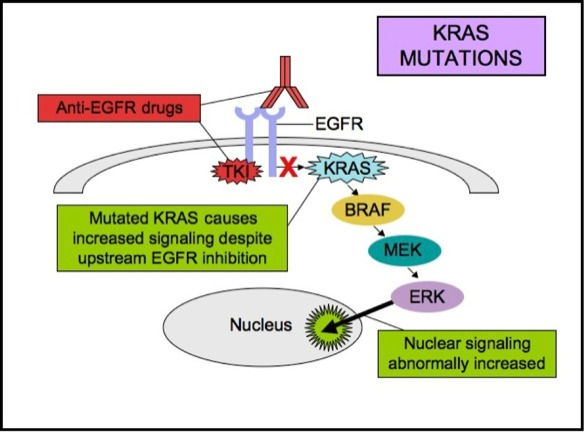
\includegraphics[height=0.72\textheight, center]{mutated_KRAS_path.jpg}

\end{frame}

%%%%%%%%%%%%%%%%%%%%%%%%%
%%%%%%%%%%%%%%%%%%%%%%%%%
%%%%%%%%%%%%%%%%%%%%%%%%%

\begin{frame}
\frametitle{Prioritize targeted therapies using drug-gene networks}

We prioritize targeted therapies by creating networks that integrate the following ({\color{orange} inputs in orange}):

\begin{itemize}
\item {\color{orange}Specific alterations found in a patient's tumor}
\begin{itemize}
\item eg G13V in KRAS, pathogenic PIK3CA mutation
\end{itemize}
\item {\color{orange}Patient's cancer type}
\begin{itemize}
\item eg Colorectal cancer
\end{itemize}
\item Biological pathways relevant to cancer type, alterations
\begin{itemize}
\item eg KEGG
\end{itemize}
\item FDA-approved targeted cancer therapies and indications
\begin{itemize}
\item biomarker, cancer type
\end{itemize}
\item Drug-gene connections (drug targets) 
\begin{itemize}
\item eg DrugBank
\end{itemize}
\item Knowledge about activity of alterations/altered gene
\begin{itemize}
\item eg gene is an oncogene
\end{itemize}

\end{itemize}

\end{frame}

%%%%%%%%%%%%%%%%%%%%%%%%%
%%%%%%%%%%%%%%%%%%%%%%%%%
%%%%%%%%%%%%%%%%%%%%%%%%%

\begin{frame}
\frametitle{Current landing page}

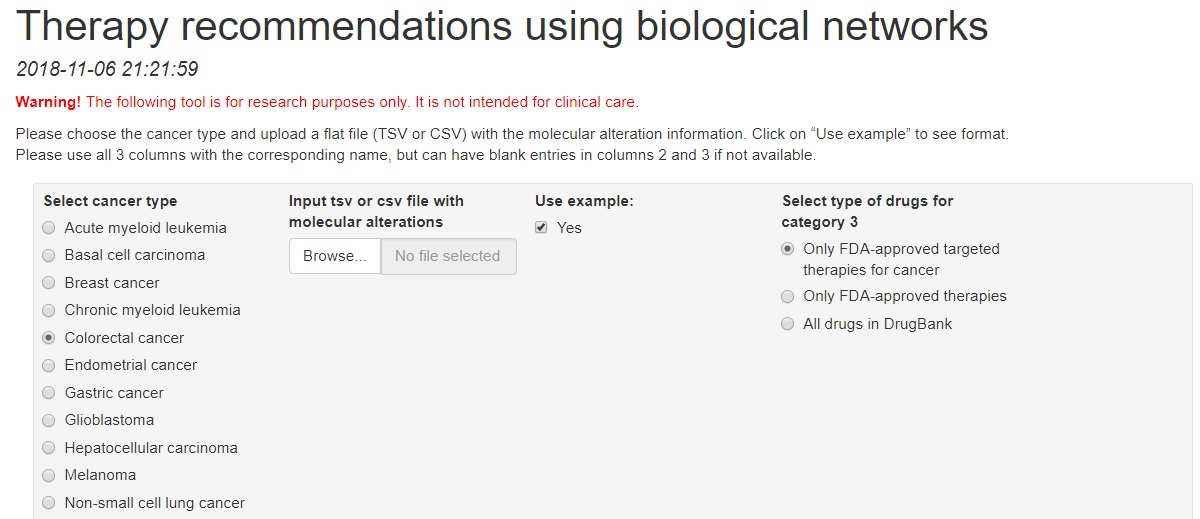
\includegraphics[width=0.95\textwidth, center]{Landing_page.jpg}

\vspace{0.4cm}

\url{https://siminaboca.shinyapps.io/Search_MP_results_using_FDA_approvals_targets_KEGG/}

\end{frame}

%%%%%%%%%%%%%%%%%%%%%%%%%
%%%%%%%%%%%%%%%%%%%%%%%%%
%%%%%%%%%%%%%%%%%%%%%%%%%

\begin{frame}
\frametitle{Allowable input format}

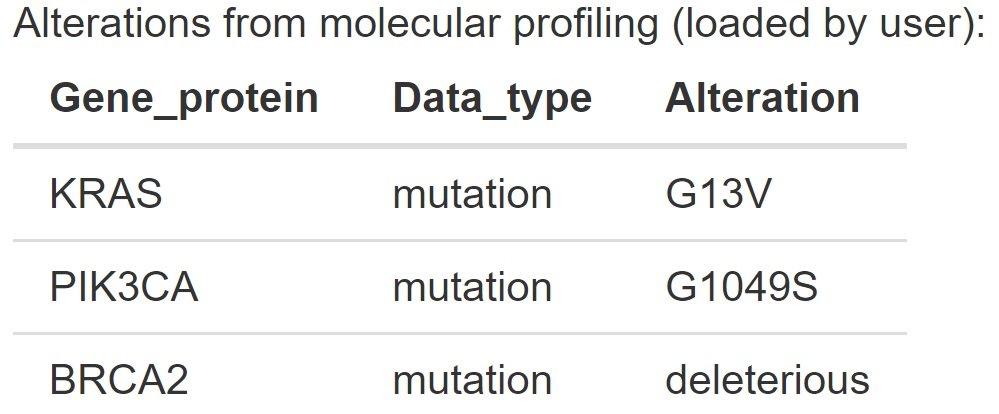
\includegraphics[width=0.90\textwidth, center]{Allowable_input.jpg}

\end{frame}

%%%%%%%%%%%%%%%%%%%%%%%%%
%%%%%%%%%%%%%%%%%%%%%%%%%
%%%%%%%%%%%%%%%%%%%%%%%%%

\begin{frame}
\frametitle{4 ordered categories of therapies}

\begin{enumerate}
\item FDA-approved drugs for which these alterations/genes/proteins are biomarkers {\color{red}in this tumor type}
\item FDA-approved drugs for which these alterations/genes/proteins are biomarkers {\color{red}in other tumor types}
\item Drugs for which these alterations/genes/proteins or others in the {\color{red}pathway corresponding to this tumor type} are targets/biomarkers*
\item Drugs for which these alterations/genes/proteins or others in {\color{red}general cancer pathways} are targets/biomarkers*

\end{enumerate}

\vspace{0.5cm}

* They could be drugs prescribed for other tumor types

\vspace{0.4cm}

When considering pathways, currently looking just at portions of pathways downstream of {\color{red}oncogenes}.

\end{frame}

%%%%%%%%%%%%%%%%%%%%%%%%%
%%%%%%%%%%%%%%%%%%%%%%%%%
%%%%%%%%%%%%%%%%%%%%%%%%%

\begin{frame}
\frametitle{Example of current ordered recommendations}

For the colorectal cancer patient with: G13V in KRAS, G1049S in PIK3CA mutation, deleterious mutation in BRCA2, the prioritization is:
\vspace{0.2cm}

\begin{enumerate}
\item {\color{red}No recommended therapy}
\item {\color{red}Olaparib and rucaparib}
\begin{itemize}
\item Approved in breast, ovarian, fallopian tube, or peritoneal cancers for BRCA2 mutations
\end{itemize}
\item {\color{red}BRAF inhibitors, MEK inhibitors}*
\begin{itemize}
\item Approved for melanoma non-small cell lung cancer with specific BRAF mutations
\item BRAF is downstream of KRAS in colorectal cancer
\item BRAF mutations are also biomarkers for MEK inhibitors
\end{itemize}
\item {\color{red}MTOR inhibitors, ERBB2 inhibitors, EGFR inhibitors}*
\begin{itemize}
\item Approved for a variety of tumors types
\item MTOR is downstream of KRAS and PIK3CA 
\end{itemize}
\end{enumerate}

\vspace{0.2cm}

* These are among the list of recommended therapies

\end{frame}

%%%%%%%%%%%%%%%%%%%%%%%%%
%%%%%%%%%%%%%%%%%%%%%%%%%
%%%%%%%%%%%%%%%%%%%%%%%%%

\begin{frame}
\frametitle{Example of category 3 recommendations}

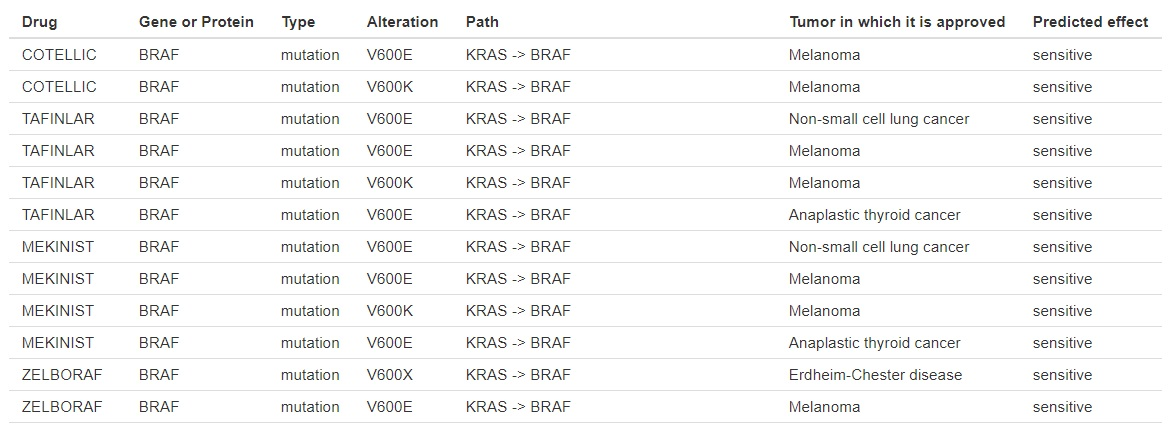
\includegraphics[width=0.90\textwidth, center]{Category_3_example.jpg}

\vspace{0.2cm}

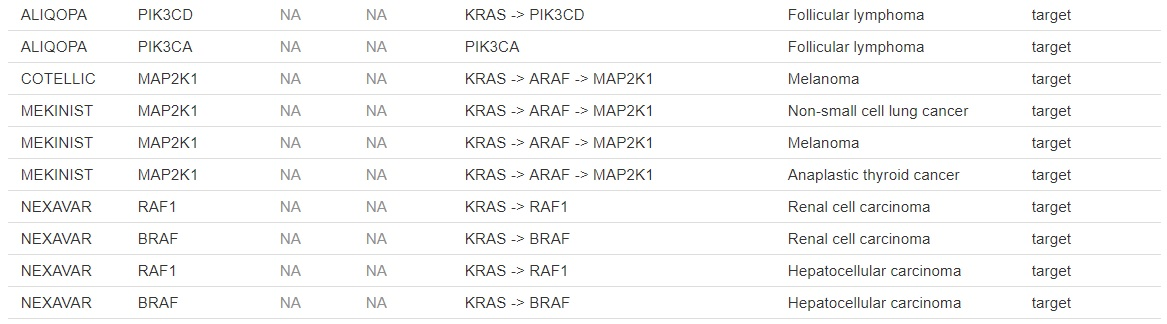
\includegraphics[width=0.90\textwidth, center]{Category_3_example_target.jpg}

\end{frame}


%%%%%%%%%%%%%%%%%%%%%%%%%
%%%%%%%%%%%%%%%%%%%%%%%%%
%%%%%%%%%%%%%%%%%%%%%%%%%

\begin{frame}
\frametitle{Standard visualization}

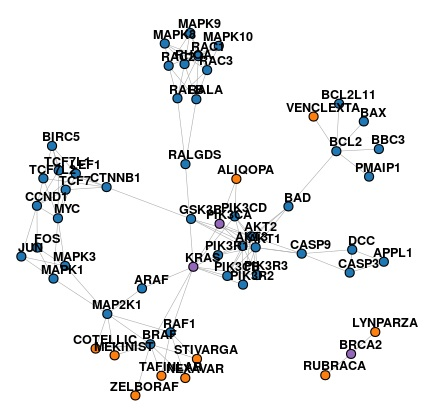
\includegraphics[width=0.70\textwidth, center]{Visualization_standard.jpg}

\end{frame}

%%%%%%%%%%%%%%%%%%%%%%%%%
%%%%%%%%%%%%%%%%%%%%%%%%%
%%%%%%%%%%%%%%%%%%%%%%%%%

\begin{frame}
\frametitle{Standard Cytoscape visualization (connection with Cytoscape under development)}

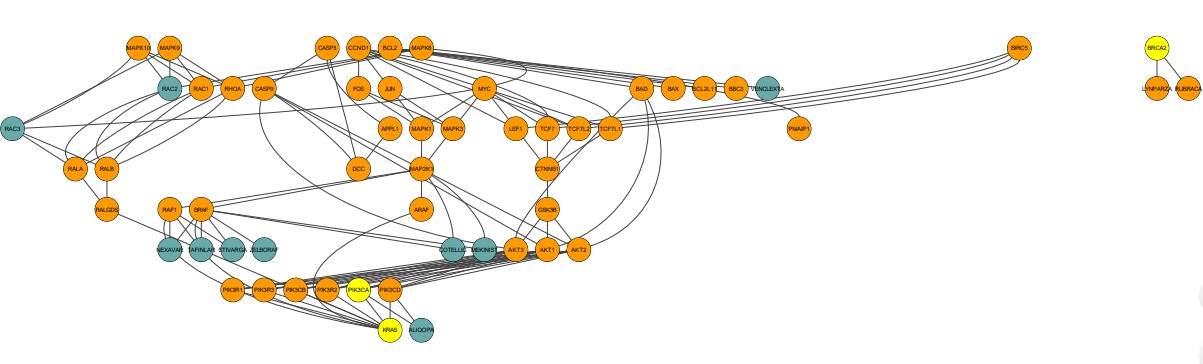
\includegraphics[width=0.80\textwidth, center]{Visualization_cytoscape.jpg}

\end{frame}

%%%%%%%%%%%%%%%%%%%%%%%%%
%%%%%%%%%%%%%%%%%%%%%%%%%
%%%%%%%%%%%%%%%%%%%%%%%%%

\begin{frame}
\frametitle{Visualization focusing on flow of evidence between drug-gene and gene-gene connections}

Users can identify evidence that leads to a recommendation in an intuitive manner and connect to PubChem for more information on specific drugs.

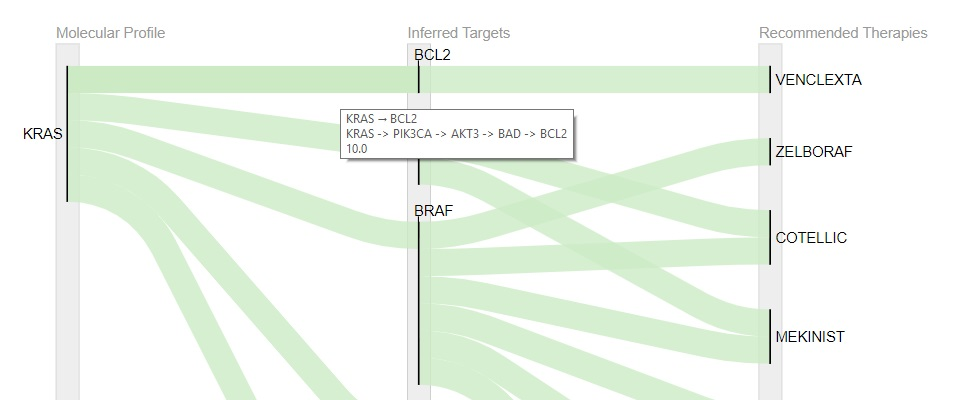
\includegraphics[width=0.90\textwidth, center]{Visualization_prototype.jpg}

\end{frame}


%%%%%%%%%%%%%%%%%%%%%%%%%
%%%%%%%%%%%%%%%%%%%%%%%%%
%%%%%%%%%%%%%%%%%%%%%%%%%

\begin{frame}
\frametitle{Current development goals}

\begin{itemize}
\item Order therapy recommendations by alteration they target
\item Incorporate information on approved drug combinations and drug classes
\item Connect to drug labels
\item Expand number of pathways used
\begin{itemize}
\item Currently just KEGG disease pathways
\end{itemize}
\item Standardize mutation types, drug names, disease names using HGVS, MeSH terms etc.
\end{itemize}

\end{frame}

%%%%%%%%%%%%%%%%%%%%%%%%%
%%%%%%%%%%%%%%%%%%%%%%%%%
%%%%%%%%%%%%%%%%%%%%%%%%%

\begin{frame}
\frametitle{Acknowledgments}

\textbf{Georgetown University:}
\begin{itemize}
\item Subha Madhavan
\item Shruti Rao
\item Robert Beckman
\item Rebecca Riggins
\item Krithika Bhuvaneshwar
\end{itemize}

\textbf{University of Maryland College Park:}
\begin{itemize}
\item Hector Corrada Bravo
\item Jayaram Kancherla
\end{itemize}

\textbf{Grant support:}
\begin{itemize}
\item R21CA220398 and R21 CA220398-02S1 (PI: Boca)
\end{itemize}

\end{frame}

%%%%%%%%%%%%%%%%%%%%%%%%%
%%%%%%%%%%%%%%%%%%%%%%%%%
%%%%%%%%%%%%%%%%%%%%%%%%%

\begin{frame}
\frametitle{Questions?}

Email: smb310@georgetown.edu \\ \vspace{0.2cm}

Twitter: \href{https://twitter.com/siminaboca}{@siminaboca}

\end{frame}

%%%%%%%%%%%%%%%%%%%%%%%%%
%%%%%%%%%%%%%%%%%%%%%%%%%
%%%%%%%%%%%%%%%%%%%%%%%%%

%%%%%%%%%%%%%%%%%%%%%%%%%
%%%%%%%%%%%%%%%%%%%%%%%%%
%%%%%%%%%%%%%%%%%%%%%%%%%

\begin{frame}[noframenumbering]
\frametitle{What is precision oncology?}

Biomarkers essentially represent tests that are used to stratify individuals into 2 or more groups.

\begin{itemize}
\item {\color{red}Predictive biomarkers} can be used to stratify patients into treatment groups with differential outcomes.\\
e.g. ``Patients with mutation X should be given treatment A instead of treatment B"
\item {\color{red}Prognostic biomarkers} are associated with different clinical outcomes for untreated or standard of care patients.\\
e.g. ``Patients with mutation X have better overall survival than patients without mutation X."
\end{itemize}

\vspace{0.6cm}

Often use the term {\color{red}``molecular profiling"} to refer to some test that considers one or more biomarkers.

\end{frame}

%%%%%%%%%%%%%%%%%%%%%%%%%
%%%%%%%%%%%%%%%%%%%%%%%%%
%%%%%%%%%%%%%%%%%%%%%%%%%

\begin{frame}[noframenumbering]
\frametitle{How should a doctor assign a targeted therapy?}

MP reports:

\begin{itemize}
\item Are used to inform choice of therapy for many cancer patients
\item Present a list of therapies predicted to lead to benefit or lack of benefit
\item Do not usually account for cross-talk within and between dysregulated pathways
\end{itemize}

\end{frame}

%%%%%%%%%%%%%%%%%%%%%%%%%
%%%%%%%%%%%%%%%%%%%%%%%%%
%%%%%%%%%%%%%%%%%%%%%%%%%

\begin{frame}[noframenumbering]
\frametitle{Parenthetical remark on evidence-based aspect}

\begin{itemize}
\item Precision medicine exemplifies the usual conflict between systematic, evidence-based analyses and
timely and available information and care
\item This tension can be seen in the lack of interaction between the systematic review (SR) and biocuration communities
\begin{itemize}
\item SRs focus on systematic analysis of literature, pay great attention to risk of bias
\item Biocuration can be much faster than SRs and presents results in more easily digestible forms
\end{itemize}
\end{itemize}

\vspace{0.4cm}

Boca SM et al. ``The future of evidence synthesis in precision oncology: Between systematic reviews and biocuration."
\textit{JCO PO}, in press. \url{http://ascopubs.org/doi/full/10.1200/PO.17.00175}

\end{frame}

%%%%%%%%%%%%%%%%%%%%%%%%%
%%%%%%%%%%%%%%%%%%%%%%%%%
%%%%%%%%%%%%%%%%%%%%%%%%%

\begin{frame}[noframenumbering]
\frametitle{Prioritize targeted therapies using drug-gene networks}

We prioritize targeted therapies by creating networks that integrate the following ({\color{orange} inputs in orange}):

\begin{itemize}
\item {\color{orange}Specific alterations found in a patient's tumor}
\item {\color{orange}Patient's cancer type}
\item Biological pathways relevant to cancer type, alterations
\item FDA-approved targeted cancer therapies and indications
\item Drug-gene connections (drug targets)
\item Knowledge about activity of alterations/altered gene
\end{itemize}

\end{frame}


\end{document}






